\documentclass[11pt,a4paper]{article}
\usepackage[T1]{fontenc}
\usepackage[utf8]{inputenc}
\usepackage{lmodern,amsmath,amssymb,amsthm,mathtools}
\usepackage[margin=26mm,headheight=15pt]{geometry}
\usepackage{microtype,booktabs,longtable,array,enumitem,graphicx}
\usepackage[dvipsnames]{xcolor}
\usepackage{fancyhdr,titlesec}
\usepackage[hyphens]{url}
\usepackage[colorlinks=true,linkcolor=MidnightBlue,citecolor=MidnightBlue,
 urlcolor=MidnightBlue,pdftitle={Compressed certificates for unknot recognition},
 pdfauthor={Research continuation for the ProveIt project}]{hyperref}
\usepackage[nameinlink,noabbrev]{cleveref}
\definecolor{ink}{HTML}{193B4B}
\definecolor{accent}{HTML}{187F86}
\titleformat{\section}{\Large\bfseries\color{ink}}{\thesection}{0.65em}{}
\titleformat{\subsection}{\large\bfseries\color{ink}}{\thesubsection}{0.65em}{}
\setlength{\parskip}{4pt}
\setlength{\parindent}{0pt}
\setlength{\emergencystretch}{2em}
\setlist{itemsep=3pt,topsep=5pt}
\pagestyle{fancy}
\fancyhf{}
\fancyhead[L]{\small\color{ink}Compressed certificates for unknot recognition}
\fancyhead[R]{\small ProveIt research}
\fancyfoot[C]{\thepage}
\renewcommand{\headrulewidth}{0.3pt}
\newtheorem{theorem}{Theorem}[section]
\newtheorem{lemma}[theorem]{Lemma}
\newtheorem{proposition}[theorem]{Proposition}
\newtheorem{corollary}[theorem]{Corollary}
\theoremstyle{definition}
\newtheorem{definition}[theorem]{Definition}
\newtheorem{example}[theorem]{Example}
\theoremstyle{remark}
\newtheorem{remark}[theorem]{Remark}
\newcommand{\Z}{\mathbb Z}
\newcommand{\F}{\mathbb F}
\newcommand{\N}{\mathbb N}
\newcommand{\Q}{\mathbb Q}
\newcommand{\poly}{\operatorname{poly}}
\newcommand{\rank}{\operatorname{rank}}
\newcommand{\supp}{\operatorname{supp}}
\newcommand{\lcp}{\operatorname{lcp}}
\newcommand{\lcsuf}{\operatorname{lcsuf}}
\newcommand{\pref}{\operatorname{pref}}
\newcommand{\suff}{\operatorname{suff}}
\newcommand{\Orb}{\operatorname{Orb}}
\newcommand{\code}[1]{\texttt{\small #1}}
\newcommand{\baseline}{\texttt{1be2abc8cc743c1a3b5cb7fdfeb650697f8e2d5b}}
\newcommand{\subtreebaseline}{\texttt{38e65c9c2e2bfd42b9f71f1a1a7af15a3f8a3005}}
% Recorded integrated suite: all tests passed with Regina 7.4.1 enabled.
\newcommand{\TestCount}{735}
\newcommand{\TestSeconds}{110.513}


\begin{document}
\hypersetup{pageanchor=false}
\begin{titlepage}
\vspace*{18mm}
{\color{accent}\large PROVEIT / TOPOLOGY / RESEARCH CONTINUATION\par}
\vspace{12mm}
{\color{ink}\Huge\bfseries Compressed certificates\par
 for unknot recognition\par}
\vspace{9mm}
{\Large Arithmetic overlap families, regular-cover gluings,\par
 and normal disks\par}
\vspace{14mm}
{\large 8 October 2026\par}
\vspace{13mm}
\begin{abstract}
We develop three exact computational improvements motivated by the remaining
gap between the maintained \code{fastunknot} implementation and a general
$n^{O(\log n)}$ recognition bound. First, a short endpoint word can identify
an arithmetic progression containing every possible suffix--prefix overlap.
An exact periodicity certificate makes candidate validity monotone in
progression rank; galloping and bisection filter the entire progression.
Its step and cardinality may both be
exponentially large in their binary descriptions. This strictly extends the
implementation's fixed short-period and bounded-marker shortcuts while
preserving the complete fallback.

Second, we give a polynomial algorithm, in the encoded input size, for
equivalence of framed assemblies of connected regular cyclic or dihedral
surface covers. A spanning forest reduces all local gluing phases to one
group element per graph component. Cycle and boundary-mark constraints become
at most two systems of congruences. We also count the remaining unmarked
classes exactly: cyclic assemblies have $m^\beta$ classes, where $\beta$ is
the cycle rank. Thus efficient equivalence testing alone does not control
the number of distinct geometric states.

Third, we implement an independent normal-disk verifier using a primitive
extreme-ray certificate, modular rank, Euler characteristic, and boundary
intersection parity. It validates the finite triangulation and never expands
the normal surface. Fibonacci layered solid tori provide an explicit
exponential-weight test family. These results include proofs, adversarial
checks, measured positive and negative outcomes, and a repository patch.
The general quasi-polynomial recognition bound remains unproved.
\end{abstract}
\vfill
{\small Research prepared for integration into
\url{https://github.com/VladimirReshetnikov/ProveIt}.\par
All new numerical claims are tied to reproducible artifacts. Classical
normal-surface and compressed-word results are credited separately from
the implementation and refinements developed here.}
\end{titlepage}
\hypersetup{pageanchor=true}
\pagenumbering{roman}
\begingroup
\small
\setlength{\parskip}{0pt}
\tableofcontents
\endgroup
\clearpage
\pagenumbering{arabic}

\section{Research status and the concrete advance}
\label{sec:status}

\subsection{What is being continued}

The maintained repository already contains a substantial exact recognizer:
structural and braid certificates, polynomial one-sided obstructions,
width-sensitive Jones and Khovanov computations, compressed group operations,
and an optional complete normal-surface backend. Its synthesis article had
reached 210 pages before this work. Repeating the existing width-conditional
recurrences, or adding another invariant with no effect on the surviving
search space, would not close its main theoretical gap.

The public checkout and preceding relevant revision are pinned as follows
\cite{proveit}:
\begin{center}\small
\begin{tabular}{@{}ll@{}}
Checkout & \baseline\\
Subtree revision & \subtreebaseline\\
Shared \code{fast/} tree & \texttt{e7222244bb0d7f35cf7f34f83228b350240e4d13}
\end{tabular}
\end{center}
The preceding subtree revision is entitled ``Document sparse endpoint proofs
and controlled overlap measurements.'' Both references have the same
maintained \code{fast/} tree. The patch is prepared against the full checkout
reference. It does not depend on remembering an earlier conversational archive.

The latest compressed-overlap implementation already had two certified
shortcuts. One recognized a common cyclic pattern with period at most 32.
The other counted occurrences of an endpoint letter, saturating at 65, and
individually verified at most 64 forced candidates. Their exact fallbacks were
complete, but long-period blocks with many repeated markers could still
exhaust the allotted work. We remove those two numerical restrictions on a
structurally certified class. The important change is from enumerating a
bounded number of candidate lengths to proving a formula for all of them.

Two geometric interfaces are developed alongside that change. The existing
surface-cover kernel describes a particular affine action on a cyclic sheet
set. It does not solve gluing equivalence for an assembly of regular covers.
The new assembly kernel has a deliberately different, checked input model.
The existing Regina wrapper exports an external-engine verdict and metadata;
it does not independently certify a supplied normal disk. The new verifier
checks such a disk in a supplied finite triangulation. These are exact
additional capabilities, with their premises visible at the interface.

\subsection{What the current literature actually supplies}

Lackenby's July 2026 preprint gives a new algorithm based on essential
hierarchies and boundary patterns \cite{lackenby2026}. Section 9 explicitly
distinguishes a bound on the number of steps from a running-time estimate for
all steps. Its later sections develop polynomial verification and compressed
decomposition when suitable surfaces are supplied. In particular, supplying
a normal surface in binary coordinates and cutting efficiently along it are
not equivalent to finding the required surfaces or bounding the complete
recognition computation. The repository correctly preserves this distinction.

Compressed-word equality and several fully compressed matching operations
already have polynomial algorithms in grammar size
\cite{schleimer,lifshits,matsubara}. The present endpoint construction is a
more economical exact route for a broad promised class of overlap queries.
We do not claim that it changes a previously exponential general compressed
matching problem into a polynomial one.

Likewise, polynomial normal-surface verification is classical. The
extreme-ray approach is part of the Hass--Lagarias--Pippenger framework
\cite{hlp}; the more general orbit-counting machinery of
Agol--Hass--Thurston handles surfaces beyond this restricted certificate
class \cite{aht}. Our contribution is a small independently inspectable
implementation, an explicit modular rank certificate, a parity test for the
boundary, and a reproducible comparison that does not require expanding a
normal disk. General normal-surface discovery remains a separate problem.

\subsection{Results and their precise scope}

\begin{longtable}{@{}>{\raggedright\arraybackslash}p{.25\textwidth}>{\raggedright\arraybackslash}p{.38\textwidth}>{\raggedright\arraybackslash}p{.30\textwidth}@{}}
\toprule
Result & Exact guarantee & Remaining premise or limitation\\
\midrule
Endpoint progressions & All suffix--prefix overlaps are returned from a
certified short-anchor occurrence progression; both its step and count are
binary integers with no fixed cap. & Failure of the structural certificate
uses the complete matcher; the inherited extension queries can still be
expensive.\\
Regular-cover gluing & All framed isomorphisms are encoded by at most two
root congruence classes per connected assembly graph. & Each block is a
connected regular cover with checked compatible whole-boundary attachments;
the blocks are already supplied.\\
Gluing state count & Exact orbit counts, including $m^\beta$ for cyclic
covers, quantify states left after relabelling. & This is a lower bound for
enumerating these framed classes, not for arbitrary unknot algorithms.\\
Normal disk certificate & A supplied finite triangulation and binary normal
vector are checked to contain an essential compressing disk. & The vector
must satisfy the extreme-ray condition; correspondence with a given PD
diagram is not asserted.\\
\bottomrule
\end{longtable}

The distinction between a complete recognizer and a complete local operation
is central. The word shortcut participates in an already existing optional
compressed group search. The gluing and normal-disk kernels are new explicit
APIs. They do not silently introduce new positive or negative knot verdicts
into the pipeline.

\section{Encodings, cost measures, and proof obligations}
\label{sec:models}

The number $n$ denotes crossings in a validated classical knot diagram,
not expanded word length or the size of an unencoded geometric construction.
We use the specific target $n^{O(\log n)}=2^{O((\log n)^2)}$. Some authors use
``quasi-polynomial'' for the larger union of bounds
$2^{(\log n)^{O(1)}}$; any use of that broader convention must be stated.

An SLP is an acyclic binary grammar whose rules are terminals or
concatenations of earlier rules. Let $g$ be the number of reachable rules,
$H$ its height, $L$ the maximum represented length, and
$B=\lceil\log_2(L+1)\rceil$. Lengths, positions, and counts are binary
integers. Signed generator names have their own bit lengths and are compared
exactly. A grammar may contain two copies of the same child in one rule;
its represented occurrence count must therefore respect multiplicity even
when the grammar nodes themselves are shared.

For surface assemblies, $m$ is the cyclic parameter, and
$\ell=\lceil\log_2(m+1)\rceil$. The regular dihedral group has order $2m$;
it is not the generally nonregular action of a dihedral subgroup on $m$
residues. Let $v,e,r$ denote the numbers of blocks, attachments, and
explicit markings, with the total listed local monodromy data included in
the input size. For a connected assembly graph, $\beta=e-v+1$.

For the normal-disk verifier, $t$ is the number of tetrahedra, $x$ the
normal coordinate vector, $s=|\supp x|\leq7t$, and $B_x$ the largest
coordinate bit length. A tetrahedron has four triangle and three
quadrilateral types. Face maps are explicit vertex permutations, not an
unverified topology label or a hash of one.

We distinguish three measurements throughout. A mathematical bit bound counts
integer operations according to operand length. The implementation's work
counter charges selected operations cooperatively; it is a resource policy,
not an exact instruction count. Wall-clock measurements are empirical and
include the scope specified by each benchmark. A resource-limited computation
has no recorded completion time. It cannot serve as the denominator of a
completion-speedup claim.

\begin{proposition}[Local bounds do not compose without state bounds]
Suppose each operation on an encoded state of size $S$ costs $S^c$ for a
fixed $c$. If a computation performs $R(n)$ charged state-processing
operations, including repeated visits, and every participating state has
size at most $S(n)$, its operation cost is bounded by
$R(n)S(n)^c$, before adding input conversion and output verification.
To obtain the target $n^{O(\log n)}$ from this estimate, it suffices to prove both
$\log R(n)=O((\log n)^2)$ and
$\log S(n)=O((\log n)^2)$, with the other work similarly controlled.
\end{proposition}
\begin{proof}
Sum the local cost over the actual operations. Taking logarithms yields
$\log R+c\log S$. The statement requires bounds for the states actually
processed and the number of processing operations; the existence of a
smaller representation, or a bound only on distinct states, is insufficient.
\end{proof}

This elementary accounting is included to locate the obligation, not as a
new recognition theorem. The gluing orbit count below gives a concrete
reason that an efficient quotient computation can leave too many distinct
states for this argument to meet the target.

\section{All overlaps from an arithmetic endpoint family}
\label{sec:overlaps}

\subsection{Candidate lengths forced by a short endpoint word}

For finite words $X,Y$, define
\[
 \mathcal O(X,Y)=\{k:1\leq k\leq\min(|X|,|Y|),\;
                    \suff_k(X)=\pref_k(Y)\}.
\]
These are literal signed-word equalities. Free reduction is not performed
inside this definition. In the application, the surrounding group algorithm
chooses the words whose overlaps are to be queried.

Write $L=\min(|X|,|Y|)$. Replacing $X$ by its last $L$ letters and $Y$ by
its first $L$ letters preserves $\mathcal O(X,Y)$. We therefore assume both
operands have length $L$. Pick $1\leq q\leq L$ and let
$P=\suff_q(X)$. Every overlap of length $k\geq q$ forces an occurrence of
$P$ in $Y$ ending at position $k$, where positions are counted from one.
Thus the set
\[
 K_P(Y)=\{i+q:Y[i:i+q]=P\}
\]
contains every possible overlap length at least $q$. This is only a necessary
condition. The algorithm must verify all lengths that it accepts.

An arithmetic progression is represented by $(a,d,c)$, denoting
$\{a,a+d,\ldots,a+(c-1)d\}$. For $c>1$, require $d>0$;
for a singleton, use $d=0$. Both $d$ and $c$ are exact binary integers.

\begin{theorem}[Endpoint progression clipping]
\label{thm:endpoint}
Suppose $K_P(Y)$ is a nonempty arithmetic progression $K$ with largest
member $M$, and put $U=\pref_M(Y)$. If $K$ has at least two members,
let its step be $d$ and suppose that $U$ has period $d$. Then
\begin{equation}
 \mathcal O(X,Y)\cap[q,L]
   =K\cap[q,\lcsuf(X,U)].
 \label{eq:endpoint}
\end{equation}
The hypothesis about the period is decidable by the exact equality
\begin{equation}
 U[0:M-d]=U[d:M].\label{eq:period-check}
\end{equation}
No periodicity hypothesis on the other operand $X$ is required.
\end{theorem}
\begin{proof}
If $K=\{M\}$, the only candidate is accepted exactly when
$\suff_M(X)=U$, equivalently when $M\leq\lcsuf(X,U)$.
Now suppose $K$ has at least two members.
Each $k\in K$ has the form $M-jd$ for an integer $j\geq0$.
The period condition implies $U[i]=U[i+jd]$ whenever both sides are within
$U$, by repeatedly applying the period identity. Therefore
\[
 \pref_k(Y)=\pref_k(U)=\suff_k(U).
\]
The condition $\suff_k(X)=\pref_k(Y)$ is consequently equivalent to
$\suff_k(X)=\suff_k(U)$, which holds precisely when
$k\leq\lcsuf(X,U)$. Conversely, every overlap of length at least $q$
belongs to $K$ by its final $q$ letters. These two implications prove \eqref{eq:endpoint}.
Equation \eqref{eq:period-check} is the definition of period $d$ for a finite word, so it gives
an exact certificate for the only periodicity used in the proof.
\end{proof}

\begin{corollary}[Symmetric endpoint direction]
\label{cor:endpoint-symmetric}
Let $Q=\pref_q(Y)$ and let
$K=\{L-i:X[i:i+q]=Q\}$. Suppose $K$ is a nonsingleton arithmetic
progression of step $d$ and maximum $M$, and $V=\suff_M(X)$ has period $d$.
Then
\[
 \mathcal O(X,Y)\cap[q,L]=K\cap[q,\lcp(V,Y)].
\]
\end{corollary}
\begin{proof}
For $k=M-jd$, periodicity gives
$\suff_k(X)=\suff_k(V)=\pref_k(V)$. Now use the definition of a longest
common prefix. The occurrence of $Q$ at the beginning of any overlap proves
necessity of membership in $K$.
\end{proof}

Empty and singleton candidate sets need separate, simpler treatment. If the
set is empty, no overlap of length at least $q$ exists. For a singleton,
one exact suffix--prefix comparison decides its membership. Every length
below $q$ is checked directly in all three cases. Hence one successful
anchor returns at most $q$ disjoint progression records: at most $q-1$
short singletons and one progression for the longer overlaps.

\subsection{Finding the cutoff by candidate rank}

The common-suffix and common-prefix lengths in the preceding statements
describe the answer, but need not be computed. A binary search for the
complete common-prefix length can examine positions that are irrelevant
to the progression. Once the progression and its period have been checked,
we can search only its candidate ranks.

\begin{corollary}[Galloping search for the last successful candidate]
\label{cor:endpoint-rank}
Under the hypotheses of \cref{thm:endpoint} or
\cref{cor:endpoint-symmetric}, write
$K=\{a+jd:0\leq j<c\}$ with $c\geq2$. Let $h$ be the number of its
members that are actual overlaps and let $z=c-h$.
All accepted members can be returned using
\begin{equation}
 O\bigl(1+\log(1+z)\bigr)
 \quad\text{exact suffix--prefix equality comparisons}.
 \label{eq:rank-comparisons}
\end{equation}
This is $O(\log(c+1))$ in the worst case. If every candidate succeeds,
one comparison suffices; if every candidate fails, at most two suffice.
These counts exclude the preceding period check and the fewer than $q$
short-length checks.
\end{corollary}
\begin{proof}
By the clipping theorem, the predicate
\[
 f(j)=\bigl[\suff_{a+jd}(X)=\pref_{a+jd}(Y)\bigr]
\]
is a true prefix: it holds precisely for $0\leq j<h$.
Check $f(c-1)$ first. If it holds, return all of $K$.
Otherwise check $f(0)$; if that fails, return the empty progression.
The remaining case has $1\leq h<c$. Maintain a checked true index
$\mathrm{lo}$ and a checked false index $\mathrm{hi}$, initially
$0$ and $c-1$.

Probe backward from the maximum at distances
$\delta=1,2,4,\ldots$, using $j=\max(0,c-1-\delta)$.
A false answer updates $\mathrm{hi}=j$; a true answer updates
$\mathrm{lo}=j$ and ends this phase. If $j=0$, its previously checked
true value supplies the endpoint without another comparison.
For an unclamped probe,
\[
 f(c-1-\delta)\text{ holds}
 \quad\Longleftrightarrow\quad \delta\geq z.
\]
Consequently the gallop uses $O(1+\log z)$ comparisons. Its final
bracket has width $O(z)$, including the clamped case. Binary search within
that bracket finds the last true index using $O(\log(1+z))$ additional
comparisons. The answer is the first $h$ members of $K$, represented by
one progression, or by a singleton when $h=1$.
The invariant also covers $c=2$, when no interior search is needed.
\end{proof}

The monotonicity is a consequence of the certified period condition.
Arbitrary overlap lengths need not have this property. The implementation
therefore applies the rank search only after the exact structural check;
it does not replace a failed period test by an assumed monotonicity.
The proof uses ordinary exponential search followed by bisection, rather
than a new general-purpose search method. Its useful feature here is the
choice of the candidate rank and the direction of the gallop.

\begin{example}[The opposite word may be nonperiodic]
Let $B$ be a word whose final letter $c$ appears nowhere else in $B$.
For integers $C\geq r\geq1$, let $Y=B^C$ and let $X=WB^r$, where
$W$ is any word of length $(C-r)|B|$. The endpoint occurrences in
$Y$ lie at $|B|,2|B|,\ldots,C|B|$. The theorem returns exactly those
multiples no larger than the actual common-suffix length. It does not need
to certify that $W$ repeats $B$, and it remains correct when $W$ contains
arbitrary defects or a partially matching suffix.
\end{example}

\subsection{Recognizing a progression without listing its points}

The missing operation is to summarize all occurrences of an explicit short
pattern in an SLP word. It is insufficient to summarize distinct grammar
nodes containing the pattern: a shared node can be used exponentially many
times in the represented word.

For an ordered finite set of occurrence starts $S$, retain
\[
 \Sigma(S)=(c,f,l,\delta_{\min},\delta_{\max}),
\]
where $c=|S|$, $f,l$ are its endpoints, and the last two entries are the
minimum and maximum consecutive gaps. Empty and singleton sets have both
gap entries zero. For $c\geq2$,
\begin{equation}
 S\text{ is an arithmetic progression}
 \quad\Longleftrightarrow\quad
 \delta_{\min}=\delta_{\max}.\label{eq:ap-test}
\end{equation}

\begin{lemma}[Exact ordered concatenation]
\label{lem:summary}
Suppose every point of $S$ precedes every point of $T$. The summary of
$S\cup T$ is determined by their summaries: counts add, the first and last
nonempty endpoints persist, and the new gap extrema are the extrema among
the old gaps and $\min T-\max S$. Translating $T$ only changes its two
endpoints. These formulas remain exact when the sets are exponentially large.
\end{lemma}
\begin{proof}
All consecutive pairs in $S\cup T$ lie within $S$, within $T$, or are the
single pair bridging their endpoints. This exhausts the gap list.
\end{proof}

For a rule $A\to BC$ and pattern length $q$, every occurrence is in exactly
one of three disjoint sets: wholly inside $B$; crossing the concatenation
cut; or wholly inside $C$. The last set is translated by $|B|$.
This locality at a grammar concatenation is standard in compressed
$q$-gram algorithms; see Goto, Bannai, Inenaga and Takeda
\cite{goto-qgrams}. The five-entry summary used here is tailored to
certifying one exact occurrence progression.
There are at most $q-1$ crossing positions. Store the first and last
$\min(q-1,|A|)$ letters of every reachable rule, and check those crossing
positions explicitly. Processing them in increasing start order allows
\cref{lem:summary} to merge all three sets without enumerating any child
occurrence set. For $q=1$ there are no crossing occurrences.

\begin{theorem}[SLP occurrence summaries]
\label{thm:summary}
For an explicit nonempty pattern of length $q$ and an SLP with $g$ reachable
rules, the occurrence summary can be computed using
$O(qg)$ stored letters and integers and
$O(q^2g+g\log(g+1))$ elementary operations with the implementation's
topological sorting. If $b$ bounds the bit length of positions, counts,
rule identifiers and signed letters, a conservative corresponding bit bound
is $O((q^2g+g\log(g+1))b)$, besides the input grammar's stored structure.
\end{theorem}
\begin{proof}
Terminal rules are immediate. The three-way partition at a concatenation
and \cref{lem:summary} establish correctness by induction on the grammar.
The retained endpoints have length at most $q-1$. There are at most $q-1$
crossing candidates, each checked against $q$ explicit letters, yielding
$O(q^2)$ elementary work per rule. The count for a repeated child is
included once on each side of the cut, correctly accounting for grammar
sharing. All integer additions, subtractions, comparisons and translations
involve $O(b)$ bits. Sorting the reachable rule identifiers adds the displayed
term; node order already respects the grammar's acyclicity.
\end{proof}

The summary is useful even when \cref{eq:ap-test} fails: it certifies that this particular
anchor does not give a single progression. It is not a complete compressed
representation of a nonprogression set. The matcher therefore tries another
anchor or falls back, rather than discarding unrepresented candidates.

\subsection{Integration and local complexity}

The implementation tries anchor sizes $1,2,4,8$, in both directions. Its
public primitive accepts other finite lists of positive sizes. A proposed
size is clipped to the available word length. The integrated hook is reached
only for a query window of length at least 128, after the earlier uniform,
short-period and sparse-endpoint shortcuts. Thus successful earlier paths
retain their previous work. The new hook is deterministic and preserves
the old complete dyadic occurrence-table fallback.

For one nonsingleton successful anchor, the implementation performs one
period equality and the candidate-rank comparisons in
\cref{cor:endpoint-rank}. It does not compute the complete longest common
prefix or suffix. Let $g$ count the rules reachable from the input operands,
let $H$ bound their height, and let $b$ bound the bit lengths of all
positions, counts, rule identifiers and signed letters involved in the
query. Write $\mathsf E(G,b)$ for a bound on one exact equality call on
an augmented grammar with at most $G$ rules, including its assertion and
cache bookkeeping. To account also for persistent arena data, let $g_0$
bound the total number of grammar rules and pre-existing equality-cache
records at entry; in particular $g_0\geq g$. Define
\[
 J=1+\left\lceil\log_2(1+z)\right\rceil.
\]
Each candidate comparison slices the same original operands. A substring
adds $O(H)$ rules and does not increase their height, so the initial
cropping, endpoint extraction, period slices, candidate slices and short
checks together create at most $O(H(q+J))$ additional rules. The equality
implementation itself uses assertions on existing rules. We may therefore
take
\[
 G=g_0+O\bigl(H(q+J)\bigr).
\]
This deliberately counts persistent data that a reachable-rule summary
does not inspect but an equality-cache cleanup might visit.
Charging $O(b^2)$ for elementary binary multiplication in the calculation
$a+jd$, a conservative bound for the new promised-class route is
\begin{equation}
 O\!\left((q^2g+g\log(g+1))b
 +(q+J)\bigl[\mathsf E(G,b)+Hb+b^2\bigr]\right).
 \label{eq:overlap-cost}
\end{equation}
The $q$ term includes the fewer than $q$ directly checked short lengths.
For the fixed list $1,2,4,8$, failed earlier anchors contribute only a
constant number of summary passes, endpoint slices and period comparisons;
the same bound applies with the largest tried $q$ and a changed absolute
constant. All large numerical dependence is through encoded lengths and
the exact comparison cost. In particular, \cref{eq:rank-comparisons}
improves the \emph{number} of comparisons; it does not make each equality
independent of the represented words. No asymptotic bound is transferred
from a different compressed-string implementation.

All calls use the same arena work allowance and cancellation callback.
Successful complete answers are cached under the caller's original root
pair, even when the actual comparison was cropped. Candidate-rank filtering
uses direct suffix--prefix comparisons in both anchor directions.
An interruption raises the existing resource exception, with no partial
overlap set entered into the answer cache.

An unsuccessful speculative certificate has a bounded number of summary
passes for the fixed policy, but its exact equality query may still be
expensive. This is why the experiments include failed period tests and
phase-shifted long-period queries. We claim the promised-class improvement
expressed in \cref{eq:overlap-cost}, not uniform dominance over every old query.

\subsection{An explicit family beyond both old numerical caps}

\begin{proposition}[Unbounded period and marker multiplicity]
\label{prop:marker-family}
For distinct signed letters $a,b,c$, positive integers $N,C$, and
$W=((ab)^Nc)^C$, let $d=2N+1$. Then
\[
 \mathcal O(W,W)=\{d,2d,\ldots,Cd\}.
\]
The $q=1$ endpoint method returns this set as a single progression, using
grammar operations polynomial in $\log(N+1)+\log(C+1)$ for its constructed
SLP. Neither $d$ nor $C$ has a fixed numerical upper bound.
\end{proposition}
\begin{proof}
The final letter is $c$, whose occurrences are exactly at multiples of $d$.
Every overlap must end at such a position in the second copy. Conversely,
each such length is a whole number of identical blocks and is an overlap.
The longest candidate window is all of $W$ and has period $d$.
Repeated squaring gives a grammar with
$O(\log(N+1)+\log(C+1))$ rules, and the exact compressed comparisons are
polynomial in that encoded grammar size.
\end{proof}

Two binary-alphabet variants demonstrate why short words are useful anchors:
\[
 W_2=((ba)^Na)^C,\qquad W_4=((ab)^Naa)^C.
\]
The terminal word $aa$ identifies exactly the block ends of $W_2$.
The terminal word $abaa$ does so for $W_4$. For $N\geq2$ the resulting
overlap sets are, respectively, the multiples of $2N+1$, and
$\{1\}$ together with the multiples of $2N+2$. The latter isolated overlap
is exactly why lengths shorter than the anchor must be retained.

With $N=C=2^{500}$, a period itself needs about 502 bits and the number of
overlaps needs 501 bits. Explicitly listing the overlaps is impossible within
reasonable resources, but their three-integer progression representation is
small. This family is a controlled compressed-string benchmark. No theorem
here says that arbitrary hard unknot instances must generate this family,
or that every important relator overlap satisfies its hypotheses.

\section{Regular-cover gluings as congruence problems}
\label{sec:gluings}

\subsection{The geometric model and why regularity matters}

Fix $G=C_m$ or $G=D_m$. We write dihedral elements as
$(\epsilon,t)=T^tR^\epsilon$, where $\epsilon\in\{0,1\}$,
$t\in\Z/m\Z$, and
\begin{equation}
 (\epsilon,t)(\eta,u)
   =(\epsilon\mathbin\oplus\eta,\;t+(-1)^\epsilon u).
 \label{eq:dihedral-product}
\end{equation}
For the cyclic group only parity zero is allowed. The order of $D_m$ is
$2m$, including the small degenerate parameters $m=1,2$.

Each block is a connected regular cover of a specified compact connected
orientable surface with nonempty boundary. Its fibre over a chosen basepoint
is identified with the set $G$, and monodromy acts by left multiplication.
The based peripheral system includes fixed paths from that basepoint to the
boundary circles. These paths are part of the coordinate framing.
The images of the supplied canonical free generators must generate all of
$G$; the implementation checks this by gcds and the presence of a reflection
in the dihedral case. This condition makes the block connected and its
monodromy action regular.

Any automorphism of one such block covering the identity on its fixed base
surface acts on the fibre by right multiplication. Indeed, a fibre map $f$
commuting with every left multiplication satisfies
$f(g)=gf(1)$ for all $g\in G$. Write it $g\mapsto gh$.
This observation is the reason one group element per block suffices.
It does not hold in this form for an arbitrary nonregular cover.

An oriented attachment edge $e:u\to v$ joins distinct available boundary
ports, possibly of the same block. Every port is used at most once. Choose
compatible reference gluings reversing the base boundary orientations. In
the fixed fibre coordinates, the two peripheral monodromies must be exact
inverses; this is checked. A phase $a_e\in G$ then glues the entire preimage
of one boundary circle to the entire preimage of the other by
$g\mapsto ga_e$ at the reference fibre. This is well-defined because right
multiplication commutes with the left peripheral action.

Thus attachments are allowed to permute the lifted boundary circles in a
specified algebraic fashion. They are not arbitrary independently chosen
permutations of individual lifts. The assembly graph is labelled and fixed,
as are the local monodromies, base surfaces, and boundary ports.
In particular, the natural dihedral action on $m$ points is generally not
the regular action on $2m$ points used here; substituting it would invalidate
the one-group-element description of all local transports.

\begin{remark}[Local and global regularity]
Every block cover is regular. The cover of the assembled base surface need
not be regular: compatible deck maps are constrained by the holonomy around
assembly cycles. The word ``regular'' in this section always describes the
local blocks and their available right multiplications.
\end{remark}

\subsection{Eliminating all tree phases}

Consider two phase assignments $a_e$ and $a'_e$ on identical local block data.
An isomorphism over the fixed labelled base decomposition consists of right
multiplications $h_v$ such that
\begin{equation}
 a_eh_v=h_ua'_e\qquad(e:u\to v).
 \label{eq:gauge}
\end{equation}
This equation follows by applying the map before or after the attachment to
an arbitrary fibre element. It is therefore both necessary and sufficient
for the local maps to glue to a global covering isomorphism.

Choose a spanning forest. For a component root $o$, let $A_v$ be the ordered
product of original phases on the tree path from $o$ to $v$, using inverses
when an edge is traversed backwards. Define $A'_v$ similarly.

\begin{theorem}[Forest reduction of gluing equivalence]
\label{thm:forest}
Every solution of the tree-edge equations is determined uniquely by one
root element $h=h_o$ and has the form
\begin{equation}
 h_v=A_v^{-1}hA'_v.\label{eq:forest}
\end{equation}
For a remaining edge $e:u\to v$, define
\[
 c_e=A_u a_e A_v^{-1},\qquad
 c'_e=A'_u a'_e(A'_v)^{-1}.
\]
The remaining conditions are exactly
\begin{equation}
 c_eh=hc'_e.\label{eq:simultaneous-conjugacy}
\end{equation}
\end{theorem}
\begin{proof}
For a tree edge traversed from $u$ to $v$, solve \eqref{eq:gauge} for $h_v$ and proceed
along the unique tree path. Reversing an edge gives the inverse formula, so
induction establishes \eqref{eq:forest} and uniqueness. Substitute \eqref{eq:forest} into \eqref{eq:gauge}, multiply
on the left by $A_u$ and on the right by $(A'_v)^{-1}$, and obtain \eqref{eq:simultaneous-conjugacy}.
The same manipulations in reverse prove sufficiency on all edges.
\end{proof}

All products here involve fixed-size group records and integers reduced
modulo $m$. The algorithm never unfolds a fibre of $m$ or $2m$ sheets.
There is also no need to try $|G|^v$ possible collections of local maps.

\subsection{At most two scalar congruence systems}

For $D_m$, write $h=(\epsilon,t)$ and fix $\epsilon$ temporarily.
If $c=(\eta,b)$ and $c'=(\eta',b')$, equation \eqref{eq:simultaneous-conjugacy} first requires
$\eta=\eta'$. If $\eta=0$, it requires
\begin{equation}
 b=(-1)^\epsilon b'\pmod m,
 \label{eq:rotation-condition}
\end{equation}
with no constraint on $t$. If $\eta=1$, it requires
\begin{equation}
 2t=b-(-1)^\epsilon b'\pmod m.
 \label{eq:reflection-condition}
\end{equation}
Let $d_2=\gcd(2,m)$. The latter is inconsistent unless its right side is
divisible by $d_2$. Otherwise it is a single congruence for $t$ modulo
$m/d_2$, obtained by dividing by $d_2$ and inverting $2/d_2$.
Only the two choices of $\epsilon$ are tried. The cyclic case has only
$\epsilon=0$ and all cycle equations are equality tests of rotation shifts.

Markings can be included without adding a branching factor per mark.
An ordered fibre-point mark $x\mapsto y$ at block $v$ requires
$xh_v=y$, and hence
\begin{equation}
 h=A_vx^{-1}y(A'_v)^{-1}.
 \label{eq:point-mark}
\end{equation}
A lifted boundary circle is an orbit $H x$ of the peripheral subgroup
$H=\langle p\rangle$. Requiring this named circle to map to $H y$ is
equivalent to
\begin{equation}
 xA_v^{-1}hA'_v y^{-1}\in H.
 \label{eq:boundary-mark}
\end{equation}
This condition preserves the specified circle without choosing a particular
point on it.

If $p=(0,r)$ is a rotation, then
$H=\{(0,jd):j\in\Z\}$, where $d=\gcd(m,r)$.
For fixed root parity, \eqref{eq:boundary-mark} first tests a parity and then is one congruence
for $t$ modulo $d$. If $p=(1,r)$ is a reflection, then
$H=\{(0,0),(1,r)\}$. The parity of the left side selects which of those
two elements is possible, leaving one congruence modulo $m$. These
derivations also handle the identity peripheral element: each boundary
circle then contains just one point of the reference fibre.

\begin{lemma}[Congruence intersection with an explicit obstruction]
\label{lem:crt}
The two conditions $t\equiv r\pmod d$ and $t\equiv s\pmod e$ are
compatible if and only if
$\gcd(d,e)\mid(s-r)$. If compatible, their intersection is one residue
class modulo $\operatorname{lcm}(d,e)$, obtainable by the extended Euclidean
algorithm. If incompatible, the failed divisibility is a certificate of
inconsistency.
\end{lemma}
\begin{proof}
Substitute $t=r+dz$. The equation $dz\equiv s-r\pmod e$ is solvable
exactly when the stated gcd divides its right side. Divide by the gcd to
obtain an invertible coefficient. The solutions differ by
$e/\gcd(d,e)$ in $z$, so by the lcm in $t$.
\end{proof}

\begin{theorem}[Complete marked gluing solver]
\label{thm:gluing}
For two checked assemblies in the model above and any explicit collection
of fibre-point and boundary-lift marks, all covering isomorphisms over the
fixed labelled base decomposition can be encoded by at most two records
per connected assembly graph. Each record has the form
\begin{equation}
 h_o=(\epsilon,r+jD),\qquad 0\leq j<m/D,
 \label{eq:root-family}
\end{equation}
where $D\mid m$. Every local transport follows from \eqref{eq:forest}. Empty branches
have independently checkable contradiction records. The algorithm has
polynomial bit complexity in the full listed input and $\log(m+1)$.
\end{theorem}
\begin{proof}
The forest theorem is exact. For each possible root parity, \eqref{eq:rotation-condition}--\eqref{eq:boundary-mark}
reduce every remaining requirement to a failed parity/equality test or a
single congruence modulo a divisor of $m$. Repeated use of
\cref{lem:crt} yields either a contradiction or precisely one residue class
modulo a divisor $D$ of $m$. Its representatives in $\Z/m\Z$ are \eqref{eq:root-family}.
There are no other solutions, since every original equation or marking was
included. Conversely, substitution proves that every reported family member
gives an isomorphism. A forest pass and a linear number of gcd, modular
inverse, and group operations use integers of $O(\log(m+1))$ bits, together
with the explicit graph and monodromy indices. Polynomial bit complexity
follows. Components are retained as a product of solution families rather
than enumerated jointly.
\end{proof}

The implementation provides two replay routes. One checks a single collection
of local transports directly against \eqref{eq:gauge} and the original marks, without
using a spanning forest or CRT. The other checks the reported complete
solution families and their contradiction records. It verifies the
congruences and their combined modulus, rather than rerunning the producer's
CRT search. These routes separate the correctness of a particular witness
from the stronger assertion that no isomorphisms were omitted.

For a more explicit bound, let $N$ count the listed vertices, edges, free
generators and marks, and let $B$ include the largest input-integer bit
length and $\log(N+2)$. After input normalization, every root residue and
modulus has $O(\log(m+1))$ bits. A conservative schoolbook bound for a
connected graph is $O(NB^3)$ bit operations, with $O(NB)$ bits of
representation. Constraint work is grouped by graph component, so the
solution-family computation has the same bound for a disconnected graph.
The implementation additionally reports the product of all component
isomorphism counts; explicitly multiplying those binary counts costs at
most another $O(N^2B^2)$ operations. No map family is enumerated.

\subsection{Canonicalization and exact residual state counts}

For an unmarked connected assembly, forest normalization makes the tree
phases identities. The remaining $\beta$ phases form a tuple in $G^\beta$;
the residual root change simultaneously conjugates this tuple. This gives
both a canonical cache representation and a count of inequivalent framed
assignments.

For $C_m$, conjugation is trivial. For $D_m$, if all tuple entries are
rotations, compare the tuple of shifts with its simultaneous negation and
choose the lexicographically smaller one. If there is a reflection, choose
the first. Its shift $a$ can be normalized to $\delta=0$ when $m$ is odd,
and to $\delta=a\bmod2$ when $m$ is even. For root parity $\epsilon$,
solve
\[
 2t=a-(-1)^\epsilon\delta\pmod m.
\]
There are at most two parity candidates for the resulting normalized tuple.
When $m$ is even, the two possible solutions differing by $m/2$ have the
same conjugation action because the half-turn is central. Taking the smaller
tuple therefore gives a polynomial-time canonical representative for this
unmarked, fixed-base equivalence relation.

\begin{theorem}[Orbit counts after all block deck changes]
\label{thm:orbits}
On a fixed connected assembly graph of cycle rank $\beta$, with compatible
local blocks and no additional marks, the number of phase assignments up to
block deck changes is
\begin{equation}
 N_{C_m}(\beta)=m^\beta.
 \label{eq:cyclic-count}
\end{equation}
For the regular dihedral model it is
\begin{equation}
 N_{D_m}(\beta)=
 \begin{cases}
 \dfrac{(2m)^\beta+(m-1)m^\beta+m2^\beta}{2m},&m\text{ odd},\\[5pt]
 \dfrac{2(2m)^\beta+(m-2)m^\beta+m4^\beta}{2m},&m\text{ even}.
 \end{cases}
 \label{eq:dihedral-count}
\end{equation}
\end{theorem}
\begin{proof}
Forest normalization identifies the desired classes with simultaneous
conjugacy orbits on $G^\beta$. This proves \eqref{eq:cyclic-count}. For a finite group,
double-count pairs consisting of a tuple and a group element fixing it:
the number of orbits is $|G|^{-1}\sum_{g\in G}|C_G(g)|^\beta$.
For odd $m$, the identity has centralizer size $2m$, the other $m-1$
rotations have centralizer size $m$, and each of the $m$ reflections has
centralizer size 2. For even $m$, the identity and half-turn have centralizer
size $2m$, the other $m-2$ rotations have size $m$, and reflections have
size 4. Substitution proves \eqref{eq:dihedral-count}, including $m=1,2$ and $\beta=0$.
\end{proof}

\begin{corollary}[When the assembled cover is regular]
\label{cor:global-regularity}
For a connected assembly graph, without imposing additional marks, the
deck group of the cover of the assembled base is isomorphic to the
simultaneous centralizer
\[
 \bigcap_{e\notin\text{forest}} C_G(c_e).
\]
The assembled cover is regular if and only if every chord holonomy $c_e$
belongs to the centre of $G$.
\end{corollary}
\begin{proof}
Set the source and target phase assignments equal in
\cref{thm:forest}. Root elements defining deck maps are exactly those
commuting with every $c_e$. Taking inverses accounts for the right-action
composition convention and identifies the deck group with this
centralizer. The assembled cover is connected and has degree $|G|$.
The deck action on a fibre is free, so it is transitive exactly when the
centralizer has order $|G|$, or equivalently is all of $G$. This is precisely
the stated centrality condition.
\end{proof}

Consequently every cyclic assembly in this model is globally regular.
For $D_m$ with $m\geq3$, the permitted central holonomies are just the
identity for odd $m$, and the identity and half-turn for even $m$.
The degenerate groups $D_1$ and $D_2$ are abelian, so all their assemblies
are globally regular. Marks can reduce the group of mark-preserving
automorphisms without changing whether the underlying cover is regular;
the criterion refers to the unmarked covering map.

\begin{corollary}[A precise enumeration obstruction]
\label{cor:gluing-obstruction}
An algorithm that explicitly lists one record for each cyclic framed gluing
class requires at least $m^\beta$ records. In particular, $\beta=1$ and
$m=2^b$ already give $2^b$ inequivalent classes, although each individual
phase and each equivalence query use only polynomially many bits in $b$.
\end{corollary}

This obstruction has a carefully limited meaning. It is not a lower bound
for unknot recognition, nor even for deciding an arbitrary property of the
assemblies. In fact, the connected underlying orientable surfaces have the
same Euler characteristic and boundary counts for fixed block and port data;
they need not be distinguished by unmarked surface homeomorphism. What grows
is the number of \emph{framed covering} classes. A hierarchy algorithm may
be able to discard some of that data, but it must prove that doing so
preserves the relevant attachments and continuations.

For an explicit graph, $\beta\leq e$ and the binary orbit count has
$O(e\log(m+1))$ bits, so exact exponentiation is polynomial in the listed
input. If a standalone caller supplies an arbitrary binary integer $\beta$,
the output itself can have exponentially many bits in $\log\beta$.
The orbit-count API must then be interpreted as output-sensitive.

\subsection{Surface topology without sheet expansion}

For each connected component of the assembly graph, its assembled covering
surface is connected because every local block is connected and every
attachment is nonempty. If the base blocks are $S_v$, then
\[
 \chi(\widetilde S)=|G|\sum_v\chi(S_v).
\]
Gluing along complete boundary circles changes no Euler characteristic.
An unused boundary port with peripheral element $p$ contributes
$|G|/\operatorname{ord}(p)$ boundary components. Thus
\begin{equation}
 b(\widetilde S)=\sum_{\text{unused ports }j}
     \frac{|G|}{\operatorname{ord}(p_j)},\qquad
 g(\widetilde S)=\frac{2-b(\widetilde S)-\chi(\widetilde S)}2.
 \label{eq:surface-topology}
\end{equation}
Right deck maps preserve the lifted orientation, and the base attachments
reverse boundary orientations, so the assembled surface is orientable.
All quantities in \eqref{eq:surface-topology} are evaluated in binary. They help audit the input
and output but do not replace the finer gluing equivalence conditions.

For a concrete nontrivial attachment, take two pair-of-pants bases with
local monodromies $T,R$ in $D_m$ and glue their reflection ports. Each
connected regular block cover has genus zero and $2m+2$ boundary circles.
The full preimages of the reflection ports consist of $m$ circles, so
the assembly has genus $m-1$ and $2m+4$ remaining boundary circles.
All its phases are equivalent because its assembly graph is a tree.
Thus even an assembly of exponentially large genus can have a small
exact comparison problem when $m$ is given in binary. The tests check this
nontrivial peripheral gluing directly against expanded sheet permutations.

\section{An independent compressed normal-disk certificate}
\label{sec:normal}

\subsection{The proposition certified by the interface}

The input to this kernel is a finite face-paired tetrahedral triangulation
$\mathcal T$ and a vector $x\in\N^{7t}$ of standard normal coordinates.
The claimed conclusion is
\begin{quote}
$\mathcal T$ is a connected compact orientable $3$-manifold with one torus
boundary, and $x$ represents a properly embedded disk whose boundary is
essential in that torus.
\end{quote}
This is a relative topological certificate. The input does not contain a knot
diagram or a verified conversion from such a diagram. Even a genuine
compressing disk does not identify an arbitrary torus-boundary manifold as a
solid torus: $(S^1\times D^2)\mathbin{\#}(S^1\times S^2)$ supplies a familiar
counterexample. For an actual knot exterior in $S^3$, a compressible boundary
does imply the unknot; establishing that this is the supplied exterior is an
additional obligation. The successful evidence object states its relative
scope explicitly.

The producer accepts a \emph{supplied} coordinate vector and tries to attach
a small rank prime. It does not enumerate surfaces. A rejected vector means
that this particular certificate format did not verify. It does not certify
incompressibility or a nontrivial knot.

\subsection{Finite triangulations are checked, not assumed}

Tetrahedra and vertices are numbered. A face record is either a boundary
marker or a destination tetrahedron together with a permutation of its four
vertices; the image of the source face is determined by that permutation.
The verifier reconstructs the quotient and checks the following conditions.

\begin{enumerate}
\item Every face pairing is reciprocal. A face is not glued to itself.
All indices and permutations have the exact declared types and ranges.
\item The graph of tetrahedra joined through paired faces is connected.
An orientation sign on every tetrahedron solves the face-orientation
equations, whose multiplier is minus the sign of the gluing permutation.
\item Edge identifications never identify an edge with its own reverse.
Each edge link has zero or two unpaired endpoints. Since its constituent
segments are joined at endpoints, and an edge equivalence class gives a
connected link, these links are circles or intervals.
\item Vertex links are reconstructed from their triangles, edges, and
vertices. The preceding local checks make them connected surfaces; their
Euler characteristics must be $2$ when closed and $1$ when they have
boundary. They are consequently spheres or disks. Ideal vertices and
nonmanifold vertices are rejected.
\item The finite boundary is connected and has Euler characteristic zero.
The checked ambient orientation induces a boundary orientation, so this
boundary is a torus.
\end{enumerate}

The vertex-link conclusion uses the classification of compact surfaces.
For a connected surface with nonempty boundary, Euler characteristic one
forces a disk even without an orientability premise. The separate edge and
link checks are essential: Euler characteristic alone does not certify that
an arbitrary two-dimensional quotient is a surface.

These checks involve $O(t)$ combinatorial cells, represented by union--find
structures and finite graphs. They are included in the measured certificate
time. No field supplied by a topology engine is trusted as a substitute.

\subsection{Normal coordinates and the support-rank certificate}

The seven coordinates in a tetrahedron are ordered
\[
 (T_0,T_1,T_2,T_3,Q_{01|23},Q_{02|13},Q_{03|12}).
\]
Triangles link vertices; the indicated quadrilateral avoids the two listed
opposite edges. The verifier reconstructs the normal matching matrix $A$,
checks $Ax=0$, and checks the quadrilateral condition: at most one of the
three quadrilateral coordinates is nonzero in each tetrahedron. Together
with $x\geq0$, these are the standard admissibility conditions for an
embedded normal surface \cite{hlp,jaco-rubinstein}.

Let $I=\supp x$, $s=|I|$, and let $A_I$ restrict the columns of $A$ to $I$.
Each face-arc matching row has two positive and two negative contributions,
before cancellations caused by identifications. Triangle and quadrilateral
columns are distinct, so its Euclidean norm is at most $2$. This bound
remains true after restricting columns.

\begin{theorem}[Primitive support-nullity certificate]
\label{thm:primitive}
Suppose $x\ne0$ is admissible, $\gcd(x_1,\ldots,x_{7t})=1$, and
$\rank_\Q A_I=s-1$. Then the represented normal surface is connected.
\end{theorem}
\begin{proof}
Write the coordinate vectors of its nonempty connected components as
$x^{(1)},\ldots,x^{(k)}$. Each is a nonnegative integer vector satisfying
the matching equations, supported in $I$, and their sum is $x$.
The one-dimensional kernel of $A_I$ therefore gives
$x^{(j)}=\lambda_jx$, with $\lambda_j>0$.
Primitivity supplies integers $b_i$ with $\sum_i b_i x_i=1$, whence
$\lambda_j=\sum_i b_i x_i^{(j)}$ is an integer. Since
$\sum_j\lambda_j=1$, there is exactly one component.
\end{proof}

This is the classical extreme-ray argument, not a new general connectivity
theorem for normal surfaces. The support condition is equivalent to the
vector lying on an extreme ray of the nonnegative matching cone. It is
stronger than merely being a connected normal disk. A connected disk outside
this class can be rejected by the present format.

\begin{lemma}[One prime certifies rational rank]
\label{lem:rank-prime}
If a checked prime $p$ satisfies $\rank_{\F_p} A_I=s-1$, then
$\rank_\Q A_I=s-1$. Conversely, if the rational rank is $s-1$, a suitable
prime occurs among the first $s$ primes.
\end{lemma}
\begin{proof}
A nonzero minor modulo $p$ is a nonzero integer minor. Thus the modular rank
is a lower bound for rational rank. The exact nonzero vector $x$ is in the
rational kernel, giving the opposite upper bound $s-1$.

For the converse, choose a nonzero $(s-1)$-minor $D$. Hadamard's inequality
and the row-norm bound give $1\leq|D|\leq2^{s-1}$. A nonzero integer in
this range has at most $s-1$ distinct prime divisors: a product of $s$
distinct primes is larger than $2^{s-1}$. At least one of the first $s$
primes does not divide $D$, and the modular rank at that prime is $s-1$.
When $s=1$, the empty minor is $1$ and rank zero is immediate.
\end{proof}

The certificate stores the prime, not a trusted assertion that it is prime.
The verifier restricts it to
\begin{equation}
 2\leq p\leq 32(s+1)^2
 \label{eq:prime-bound}
\end{equation}
and proves primality by exact trial division. This deliberately generous
bound keeps even that elementary test polynomial in the encoded input size.
An adversary cannot turn verification into trial division of an arbitrary
binary integer.

Here is an elementary supply proof for \eqref{eq:prime-bound}. Put
$N=32(s+1)^2$ and let $\pi(N)$ count primes at most $N$. The central
binomial coefficient satisfies
\[
 \frac{2^N}{N+1}\leq \binom{N}{N/2}\leq N^{\pi(N)}.
\]
For the upper bound, Legendre's formula shows that each term in the
$p$-adic valuation is zero or one. Hence the full contribution of a prime
$p$ to the binomial coefficient is at most
$p^{\lfloor\log_pN\rfloor}\leq N$. Consequently
\[
 \pi(N)\geq\frac{N-\log_2(N+1)}{\log_2N}>s.
\]
For completeness, $N-\log_2(N+1)\geq N/2$ here and
$\log_2N=5+2\log_2(s+1)\leq5+2s$; therefore the last quotient is at
least $16(s+1)^2/(5+2s)>s$.

\begin{corollary}[Coordinate size on the certified ray]
\label{cor:coordinate-size}
For a primitive vector with this support-nullity property,
every positive coordinate is at most $2^{s-1}$. The coordinates therefore
have $O(t^2)$ total bits.
\end{corollary}
\begin{proof}
Choose $s-1$ independent rows of $A_I$. Their signed maximal minors form
a nonzero integer kernel vector. Dividing by their common divisor gives
the primitive kernel generator, up to sign. Each minor has absolute value
at most $2^{s-1}$ by the same row-norm estimate. There are at most $7t$
coordinates, each with $O(t)$ bits.
\end{proof}

This is a certificate-size statement. It does not say that an algorithm can
find the ray without examining exponentially many possible supports or
quadrilateral choices.

\subsection{Euler characteristic without expanding the surface}

Let $w_e$ denote the intersection number with a global triangulation edge.
In local edge $ab$ of tetrahedron $i$, it is
\[
 w_{ab}=T_a+T_b+Q_{01|23}+Q_{02|13}+Q_{03|12}-Q_{ab|cd},
\]
where $cd$ is the opposite edge. All local representatives of a global
edge must give the same value; the verifier checks this directly.
The normal arc count on face $f$ is
\[
 a_f=\sum_{v\ne f}T_v+\sum_Q Q.
\]
Counting each paired face once and each boundary face once gives
\begin{align*}
 V_S&=\sum_{e\text{ global}}w_e,\\
 E_S&=\sum_{f\text{ paired once}}a_f+
       \sum_{f\text{ boundary}}a_f,\\
 F_S&=\sum_i x_i,\qquad \chi(S)=V_S-E_S+F_S.
\end{align*}
These are the cells of the normal surface induced by the triangulation,
computed through their binary multiplicities. The checker requires
$\chi(S)=1$ and a positive boundary-arc count. Combined with
\cref{thm:primitive}, the classification of surfaces gives a disk. No
independent orientability test on the normal surface is required for this
particular conclusion.

\subsection{Essential boundary from intersection parity}

The remaining disk could be boundary-parallel. To exclude it, assign to
each boundary edge the parity
\[
 c(e)=w_e\bmod2.
\]
For every boundary triangle, the sum on its three edges is zero: each
normal arc contributes two endpoints. Thus $c$ is a cellular cocycle,
the mod-$2$ Poincar\'e dual of the boundary multicurve. The implementation
checks this identity as well as deriving the counts from the coordinates.

A cocycle on this finite cell structure is a coboundary precisely when
there is a vertex potential $\phi$ satisfying
\[
 c(uv)=\phi(u)+\phi(v)\pmod2
 \label{eq:potential}
\]
on every boundary edge. A graph traversal assigns potentials and detects
inconsistent equations. Loop edges are retained; on a one-vertex torus
they can carry all the information.

\begin{lemma}[Parity detects essential disk boundary on a torus]
\label{lem:boundary-parity}
Once the surface has been proved to be a disk, its boundary is essential
in the checked torus if and only if $c$ is not a coboundary.
\end{lemma}
\begin{proof}
The disk has exactly one simple boundary curve. A null-homotopic simple
curve in a torus has zero integral homology class. An essential simple
curve has a primitive nonzero class $(a,b)\in\Z^2$. A primitive pair
cannot have both entries even, so its image in $H_1(T^2;\F_2)$ is nonzero.
Poincar\'e duality identifies that class with $[c]$ in cohomology.
\end{proof}

The order of these conclusions matters. For an arbitrary disconnected
normal surface, essential parallel boundary curves can cancel modulo two.
Conversely, positive Euler characteristic alone can combine several
components in misleading ways. Connectedness, disk type, and the single
torus boundary are proved before parity is interpreted topologically.
The code can calculate intermediate values in a different order, but it
returns success only after every condition is satisfied.

\begin{theorem}[Soundness and bit complexity of the disk verifier]
\label{thm:disk}
Acceptance of the face pairing, coordinate vector, and rank prime proves
the relative proposition at the start of this section. With schoolbook
integer arithmetic, a conservative bound for one verification is
\[
 O\bigl(tB_x^2+t^3\log^2(t+2)\bigr)
\]
bit operations and polynomial space. No term is proportional to
$\sum_i x_i$.
\end{theorem}
\begin{proof}
The finite combinatorial checks establish the ambient manifold and its
boundary. Matching and quadrilateral admissibility establish the embedded
normal surface. The modular rank and primitivity prove connectedness;
Euler characteristic and boundary count prove disk type; the nonzero
parity class proves essential boundary.

There are $O(t)$ coordinate and matching operations on $B_x$-bit integers.
The gcd computations can be bounded by $O(tB_x^2)$. Dense elimination on
an $O(t)$ by $O(t)$ matrix uses $O(t^3)$ operations modulo a prime of
$O(\log(t+2))$ bits, including the lower-order pivot inversions and prime
validation. The finite topology and parity traversals are smaller terms.
All surface multiplicities are stored and manipulated as binary integers.
\end{proof}

The implementation specializes $p=2$ to packed exact XOR elimination.
The producer may try $s$ primes, so its rank work can be larger by that
factor; the certificate verifier performs only one rank check. None of
this replaces the more general orbit-counting algorithms of
Agol--Hass--Thurston \cite{aht}. It is a compact certificate format for
the primitive extreme case, with a small independent trusted computation.

\subsection{An explicit exponential-weight fixture family}
\label{sec:fibonacci}

Let $F_0=0$, $F_1=1$, and $F_{r+2}=F_{r+1}+F_r$. Fibonacci growth in
layered solid tori is classical \cite{jaco-rubinstein}. We record a fully
specified family because it makes the difference between coordinate size
and expanded surface size directly reproducible.

For $t\geq1$, number tetrahedra $0,\ldots,t-1$ from the boundary inward.
For $i<t-1$, face $0$ of tetrahedron $i$ is paired to tetrahedron $i+1$
by the permutation $(2,1,3,0)$, and face $1$ is paired by
$(0,3,1,2)$. A tuple here lists the images of vertices $0,1,2,3$; it is
not cycle notation. At the core, face $0$ is glued to face $1$ of the same
tetrahedron by $(1,2,3,0)$. Every inverse pairing is included. Faces $2$
and $3$ of tetrahedron $0$ are the two boundary faces. These are the
standard layered solid tori with meridian boundary intersection numbers
$F_{t+1},F_{t+2},F_{t+3}$.

In tetrahedron $i$, put $r=t-i$ and set
\begin{equation}
 x_i=(F_{r+1},F_{r+1},0,0,0,0,F_r).
 \label{eq:fibonacci-vector}
\end{equation}
On this support, write the three nonzero variables as $a_i,b_i,c_i$.
The core matching equations impose $a_{t-1}=b_{t-1}=c_{t-1}$.
The interlayer equations impose
\[
 c_i=a_{i+1}=b_{i+1},\qquad
 a_i=a_{i+1}+c_{i+1},\qquad
 b_i=b_{i+1}+c_{i+1}.
\]
They have a one-dimensional solution space over every field; all remaining
restricted matching equations are satisfied by this recurrence. Hence
the support has rank $3t-1$ even modulo two. The core coordinate is one,
so the vector is primitive. In particular the certificate prime can always
be $2$ for this family.

The exact number of elementary normal disks is
\begin{equation}
 D_t=\sum_{r=1}^{t}(2F_{r+1}+F_r)
     =\sum_{r=1}^{t}F_{r+3}=F_{t+5}-5.
 \label{eq:disk-count}
\end{equation}
The global triangulation edges have weights
$F_2,F_3,\ldots,F_{t+3}$: the core gives $1,2,3$, and each new layer
adds the next Fibonacci weight while retaining the previous global edge
weights. Therefore
\[
 V_S=\sum_{k=2}^{t+3}F_k=F_{t+5}-2.
\]
The core paired face contributes $2$ surface edges, the two paired faces
at level $r\geq2$ contribute $2F_{r+2}$, and the two outer boundary
faces contribute $2F_{t+3}$. Hence
\[
 E_S=2+2\sum_{r=2}^{t}F_{r+2}+2F_{t+3}
     =2F_{t+5}-8,
\]
including the empty sum for $t=1$. These formulas give $\chi(S)=1$.
There are $2F_{t+3}>0$ boundary normal arcs. The boundary has one vertex
and three edges. Its consecutive Fibonacci edge counts are not all even,
so the parity cocycle cannot be a coboundary. This proves the certificate
conditions for every $t$ without an expansion.

Thus $D_t=\Theta(\varphi^t)$, where
$\varphi=(1+\sqrt5)/2$, while the full coordinate vector has only $O(t^2)$
bits. The fixture generator is independent of Regina. The benchmark also
compares the generated face pairings and coordinates with Regina's native
layered-solid-torus construction for twelve small values, and retains
the supplied inputs for all measured sizes.

At $t=128$, the exact value of $D_t$ is
\[
 2\,791\,715\,456\,571\,051\,233\,611\,642\,548.
\]
The verifier manipulates the 896 coordinate positions, not that many
individual disks. This is a test of certificate checking for a supplied
triangulation, not a knot-diagram family with a demonstrated recognition
speedup.

\subsection{API and integration boundary}

The module \code{fastunknot/normal\_disk\_certificate.py} exposes a
producer, a Boolean verifier, and an evidence-producing audit function.
A certificate contains exactly a version, the coordinate rows, and a rank
prime. The audit reconstructs the matrix and every topological count; it
does not accept a supplied rank, Euler characteristic, component count,
or boundary-homology answer.

Cooperative cancellation exceptions propagate to the caller. Strict schema
validation rejects Boolean values in integer positions and malformed face
maps. Unit tests include valid disks, boundary-parallel vertex-linking
disks, nonprimitive multiples, annuli, mismatched coordinates, conflicting
quadrilaterals, invalid moduli, disconnected input, and relabelled copies.

The natural next integration is a transcript from a validated PD diagram
to its finite compact exterior triangulation, together with a checker for
that transcript. A producer may then be delegated to a fast topology
engine while the positive answer is independently replayed. This work
does not attach an unverified triangulation hash to a PD diagram and call
that replay complete.

\section{Reproducible experiments and negative evidence}
\label{sec:experiments}

\subsection{Protocol and the meaning of a recorded time}

The recorded environment is Python 3.12.14 on Linux x86-64, with
Regina distribution 7.4.1 (engine version string 7.4) for the optional native
comparisons. The measurements were made in a shared execution environment,
not on a frequency-controlled dedicated benchmark machine. The artifacts
retain individual measurements, random seeds, input data, result status,
and source digests. Small timing differences should not be interpreted as
stable effects.

The endpoint and normal-disk studies use five shuffled measured rounds after
one excluded warmup. The gluing study uses seven shuffled rounds and an
additional same-algorithm control. Every completed answer is checked outside
the timing interval where the benchmark explicitly separates an oracle.
For endpoint queries, the interval includes constructing a fresh word arena
and performing the requested operation. Both arms use the same arena,
relation-move code, and replayer; only the archived versus updated
\code{CommonSubstring} implementation is exchanged.

Unless otherwise labelled, a time is the median of completed measurements
for that arm. A paired ratio is the median of the within-round baseline/new
ratios, so it need not equal the ratio of two separately computed medians.
We give ratios only when every measured run of both arms completed. The raw
endpoint JSON also records time spent reaching a resource limit; that field
is elapsed time to interruption and is never treated here as a completion
time.

All endpoint kernel and relation-operation cases use a shared work allowance
of 2,000,000 and an arena-node allowance of 100,000. A resource failure is
reported as LIMIT. It is neither an empty overlap set nor a negative knot
decision. Work counts are implementation-defined cooperative charges, useful
for explaining a particular change but distinct from the bit model in the
proofs.

\subsection{Endpoint progressions: completed cases and remaining failures}

There are 27 kernel cases: nine families at binary exponent parameters
$b=8,32,500$. Except for the named fixed-marker controls, the repeated block
and repetition count use $N=C=2^b$. The archived baseline completes
13 of 27 cases under the fixed allowance; the rank-based version completes
25 of 27. An independent containment, disjointness, and cardinality oracle
checks each expected progression without enumerating its members.

\begin{table}[htbp]
\centering\small
\begin{tabular}{@{}lrrrr@{}}
\toprule
Kernel, $b=8$ & Baseline (ms) & New (ms) & Paired ratio & Anchor $q$\\
\midrule
65 marked blocks & 148.225 & 0.574 & $290.4\times$ & 1\\
Single-letter marker power & 231.578 & 0.711 & $318.8\times$ & 1\\
Binary bigram marker power & 204.855 & 0.830 & $259.2\times$ & 2\\
Binary fourgram marker power & 209.057 & 0.954 & $219.2\times$ & 4\\
Phase-compatible prefix & 35.938 & 0.636 & $57.4\times$ & 1\\
Nonperiodic opposite word & 232.038 & 0.799 & $290.4\times$ & 1\\
Rejected period, fallback & 242.316 & 249.324 & $0.983\times$ & --\\
\bottomrule
\end{tabular}
\caption{All five rounds complete in both arms for these rows. The last row
records the cost of trying and rejecting the certificate, not an improvement.
Times and ratios have different aggregation rules as stated in the protocol.}
\label{tab:endpoint-small}
\end{table}

The new family is not limited to an expanded period of 32 or 64 individually
checked occurrences. In the $b=500$ power tests the period needs 502 bits
and the occurrence count needs 501 bits. The following are completed new-arm
measurements; the baseline reaches its work limit in every corresponding
case, so no completion ratio is available.

\begin{table}[htbp]
\centering\small
\begin{tabular}{@{}lrrr@{}}
\toprule
Kernel, $b=500$ & New median (ms) & Charged work & Arena rules\\
\midrule
Single-letter marker power & 30.043 & 47,299 & 2,003\\
Binary bigram marker power & 40.713 & 65,358 & 2,003\\
Binary fourgram marker power & 51.875 & 97,977 & 2,006\\
Nonperiodic opposite word & 38.093 & 61,831 & 2,507\\
\bottomrule
\end{tabular}
\caption{Binary-described progressions with exponentially many candidate
lengths. Work and node counts are deterministic on these fixtures; timing
is empirical. The three power rows each need one candidate-rank comparison;
the nonperiodic-opposite row needs three.}
\label{tab:endpoint-huge}
\end{table}

The nonperiodic-opposite example is an informative ablation. An earlier,
mathematically correct implementation evaluated the whole longest common
extension in letter coordinates, then clipped the progression. At $b=500$
it exhausted the same work allowance. The final implementation observes
that only the largest candidate fails and settles the cutoff with three
candidate equalities. Both the earlier implementation and its original
benchmark harness are archived, with an explicit mapping from the historical
source names to their archived copies. This separates the benefit of the
progression theorem from the additional benefit of searching its ranks.

The damaged-period family deliberately has regularly spaced markers but
unequal intervening blocks. The period certificate rejects it. At $b=32$
and $b=500$, both implementations still reach the work limit in the complete
fallback. This is the two-case remainder in the 25/27 completion result.
Regularly spaced anchors alone are not enough to accept an overlap formula.

The already successful short-period and 17-marker controls do not enter
the new shortcut. Their work counts and arena-node counts match exactly
between arms. The same holds for shared-subword LCS, shared-subword relator,
and quotient controls. Their small wall-time variations provide context
for the much larger activated effects; they are not reported as independent
algorithmic improvements.

\subsection{Downstream word operations improve, but not every large case}

The 15 operation cases include three unaffected control families and two
phase-shifted families at each exponent size. The baseline completes
10 cases; the new implementation completes 13. A cyclic-relator case
includes rejection of a whole-donor move, finding a cyclic overlap, and
applying the resulting move with exact checks. It is a local presentation
operation, not an entire unknot-recognition run.

\begin{table}[htbp]
\centering\small
\begin{tabular}{@{}llrrr@{}}
\toprule
Operation & $b$ & Baseline & New median & Endpoint hits\\
\midrule
Phase-shifted LCS & 8 & 613.197 ms & 30.123 ms & 2\\
Phase-shifted LCS & 32 & LIMIT & 575.516 ms & 2\\
Phase-shifted relator move & 8 & LIMIT & 102.952 ms & 8\\
Phase-shifted relator move & 32 & LIMIT & 1,735.274 ms & 8\\
Phase-shifted LCS & 500 & LIMIT & LIMIT & 1\\
Phase-shifted relator move & 500 & LIMIT & LIMIT & 1\\
\bottomrule
\end{tabular}
\caption{Exact operations downstream of the overlap query. Endpoint hits
count successful local certificates even when subsequent work prevents the
whole operation from completing. A LIMIT entry has no completion time.}
\label{tab:operations}
\end{table}

For phase-shifted LCS at $b=8$, the median paired ratio is $19.83$.
At $b=32$, the relator operation completes with 1,866,801 charged work
units; the archived letter-extension ablation still reaches the allowance.
At $b=500$, a successful endpoint query does not prevent later inherited
matching and equality work from exhausting the budget. These retained
failures motivate work on the exact comparison backend and amortized grammar
growth, rather than a claim that all compressed relator operations are now
inexpensive in practice.

\subsection{Actual knot-diagram runs show no shortcut activation}

The complete-recognition comparison uses twelve existing survivor diagrams,
two mirrors, and the repository's Gordian example. Inputs are rebuilt from
their PD codes so that braid-source provenance cannot provide a hidden
shortcut. All 15 cases return UNKNOT in both arms. Their certificate digests
and recorded compressed-search statistic dictionaries agree, and the new
endpoint trial and hit counts are zero throughout.

The sums of per-case median wall times are 1.649 seconds for the archived
arm and 1.758 seconds for the updated arm. These sums are descriptive, not
a single paired-trial statistic. The Gordian case contributes most of the
time and has a broad timing spread despite identical executed search
statistics. No end-to-end knot speedup is demonstrated, and this variation
is not assigned to a shortcut that was never entered. The local positive
results remain useful implementation advances, but a knot-level performance
claim requires an activated knot-derived workload.

\subsection{Regular-cover arithmetic at very large binary degrees}

The independent literal-sheet oracle checks 3,480 comparisons: 3,410
equivalent and 70 inequivalent. These include 3,360 individual boundary-lift
pair queries and 120 random marked graphs with loops, parallel edges, and
disconnected components. Across them, 13,587 accepted literal gauge tuples
agree with the compact output families. Exhaustive orbits on all 455 phase
assignments of cycle rank two for $C_m$ and $D_m$, $1\leq m\leq6$, agree
with both the canonical keys and \cref{thm:orbits}.

The timing family has 64 blocks and 32 named boundary lifts. Modulus bit
length ranges from 39 to 24,007; a tree uses 63 edges and the cycle-constrained
graph uses 80. Input generation and hashing are excluded. Full comparison
includes raw-schema validation, monodromy and peripheral validation, marking
validation, and solving. Prepared comparison starts from checked models.

\begin{table}[htbp]
\centering\small
\begin{tabular}{@{}lrrr@{}}
\toprule
24,007-bit modulus & Full comparison (ms) & Prepared (ms) & Family count\\
\midrule
Tree with boundary constraints & 5.564 & 1.279 & 1\\
Graph with cycle constraints & 6.687 & 2.470 & 1\\
\bottomrule
\end{tabular}
\caption{Medians of seven rounds. The one tree family represents exactly
$2^{23999}$ compatible isomorphisms, and the one cycle-constrained family
represents two. No sheet expansion is attempted at these sizes.}
\label{tab:gluing}
\end{table}

\begin{figure}[htbp]
\centering
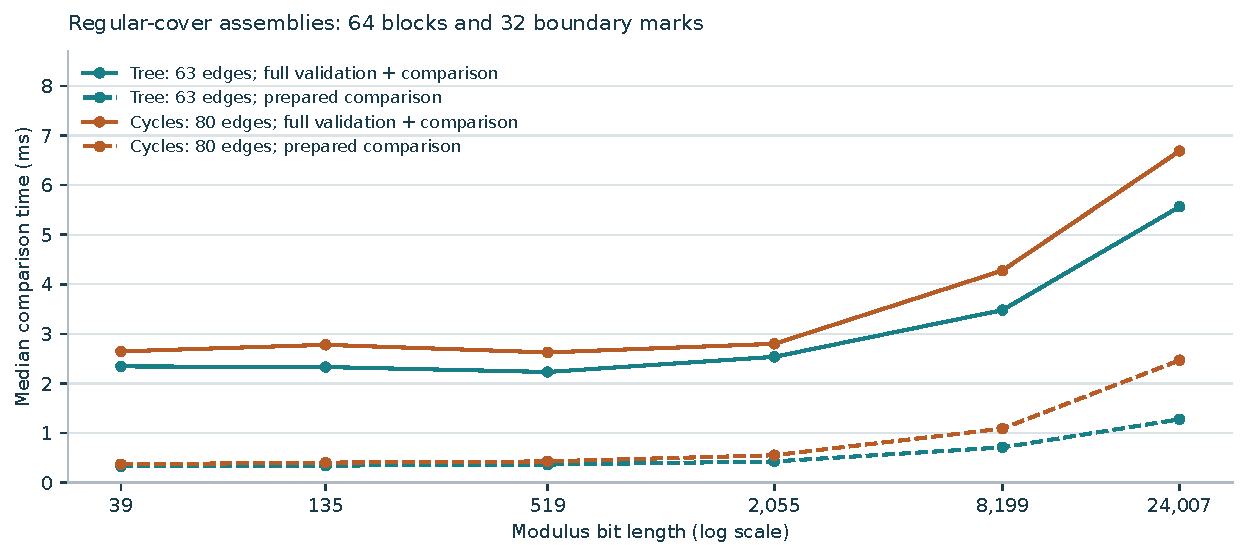
\includegraphics[width=\textwidth]{figures/gluing_scaling.pdf}
\caption{Observed gluing times as the binary modulus grows. Lines connect
measured medians and are not fitted complexity laws. The same-algorithm
control ratios range from 0.952 to 1.496; the study therefore supports
feasibility on huge encoded degrees, not precise small-factor speed claims.}
\label{fig:gluing}
\end{figure}

The exhaustive oracle is intentionally confined to small degree. There is
no measured expanded baseline at a 24,007-bit modulus, and the article
does not invent one by extrapolation. The proof supplies the reason the
compact computation avoids sheet enumeration.

\subsection{Normal disks: supplied witnesses of exponential weight}

The independent checker accepts every saved Fibonacci fixture from one
through 256 tetrahedra. For comparison, fresh worker processes call
Regina's \code{isCompressingDisc(True)} on the same supplied surfaces.
The flag gives the native predicate the advantage of assuming connectedness;
the independent checker proves it, and also validates the ambient
triangulation. Native process startup, import, and input construction are
excluded from its predicate clock. The native API documentation explicitly
describes cutting and retriangulating, with large-coordinate memory costs
\cite{regina}; this is a comparison against that API, not against the
best known theoretical normal-surface algorithms.

\begin{table}[htbp]
\centering\small
\begin{tabular}{@{}rrrrl@{}}
\toprule
$t$ & Elementary disks $D_t$ & Checker (ms) & Native (ms) & Paired ratio\\
\midrule
6 & 84 & 0.410 & 0.614 & $1.36\times$\\
10 & 605 & 0.782 & 4.924 & $7.06\times$\\
14 & 4,176 & 0.924 & 44.903 & $49.37\times$\\
18 & 28,652 & 1.173 & 414.236 & $353.25\times$\\
22 & 196,413 & 1.689 & -- & 5/5 memory failures\\
32 & 24,157,812 & 2.090 & -- & not attempted\\
64 & $\approx1.177\cdot10^{14}$ & 4.168 & -- & not attempted\\
128 & $\approx2.792\cdot10^{27}$ & 9.778 & -- & not attempted\\
256 & $\approx1.571\cdot10^{48}$ & 24.943 & -- & not attempted\\
\bottomrule
\end{tabular}
\caption{Supplied normal-surface verification, not surface discovery or
diagram-level recognition. Every checker row completes in all five rounds.
The native 22-tetrahedron runs raise MemoryError under the 768 MiB process
address-space cap. Exact large integers are retained in the fixtures.}
\label{tab:normal}
\end{table}

Native workers have a three-second allowance and a 768 MiB address-space
limit. The 22-tetrahedron failures are memory failures, not completed
predicates at the limit. For 256 tetrahedra the maximum coordinate has 178
bits, and the complete serialized input plus certificate is 69,434 bytes.
The interval includes reconstructing the finite manifold, matching,
primitivity, rank, Euler characteristic, and boundary parity. No expansion
proportional to $D_t$ occurs.

\begin{figure}[htbp]
\centering
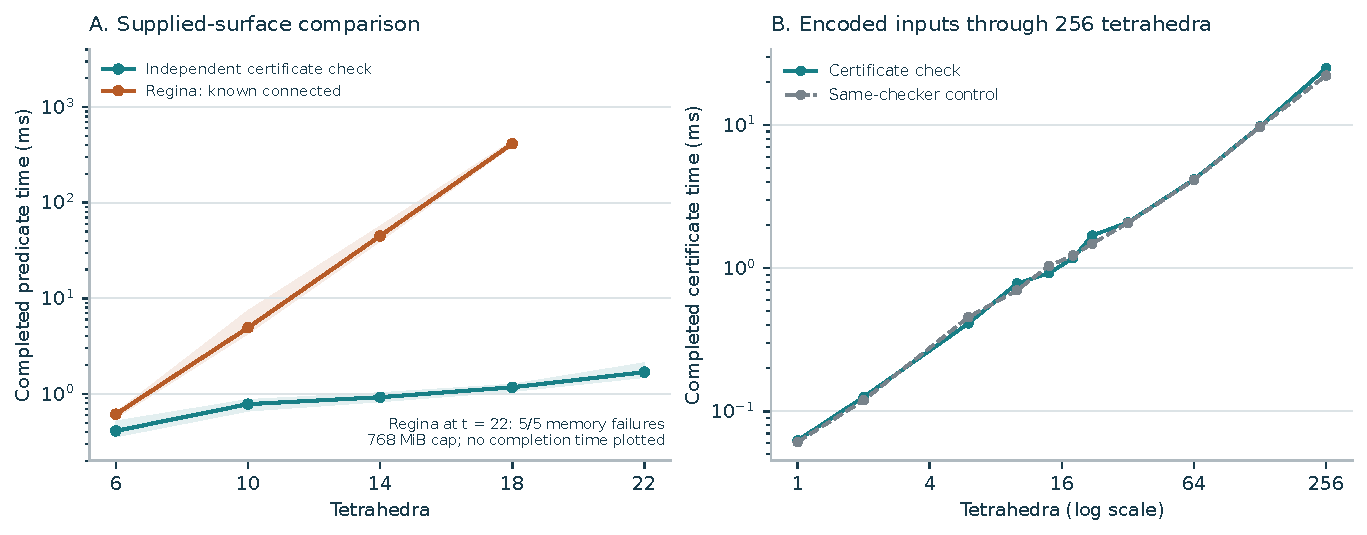
\includegraphics[width=\textwidth]{figures/normal_verification.pdf}
\caption{Normal-disk experiment. Panel A compares completed predicates;
shading is the observed range of five samples, not a confidence interval.
Panel B shows the checker and a same-checker control through the largest
saved input. The proof, rather than a regression fitted to these points,
establishes polynomial dependence on encoded input size.}
\label{fig:normal}
\end{figure}

The independent ambient-manifold audit samples 1,200 finite face-pairing
inputs with one to five tetrahedra. The checker and Regina both accept
58 as connected compact orientable manifolds with one torus boundary,
with zero mismatches. Accepted raw inputs are retained. Twelve native
layered-solid-torus constructions agree with the independent fixture
generator. In addition, 128 single-coordinate mutations are rejected, and
boundary-parallel vertex-linking disks are rejected by the parity condition.
These tests strengthen implementation confidence; the soundness theorem
does not rest on the random sample.

\subsection{Integrated validation and release structure}

The final integrated test run passes all \TestCount{} tests in
\TestSeconds{} seconds, with Regina enabled and no skipped tests.
The complete log is included. The new endpoint,
regular-cover, and normal-disk test modules contain 10, 14, and 12 tests,
respectively; individual tests often perform exhaustive or randomized
comparisons over many inputs. Historical reference implementations needed
by the maintained tests are included in their original relative paths.

Integration also exposed an existing worker-communication defect on the
tested Python runtime. Retrying a timed \code{communicate(None)} could leave
a large partially written stdin payload unsent, causing an otherwise simple
worker to time out. The original 500,000-byte regression reproduced this
failure. The correction makes one public \code{communicate(payload)} call
in an I/O thread while the caller polls cancellation and the absolute
deadline. Cleanup reaps the child, joins that thread, and closes the pipes.
Two additional regressions cover large simultaneous output and cancellation
with blocked input. This compatibility correction does not contribute to
the measured kernel gains, and is identified separately in the patch.

The release contains the complete article source, its compiled PDF, figure
sources and figures, the runnable maintained \code{fast/} code and tests,
the necessary historical test oracles, new fixtures and raw measurements,
an integration note, a patch against the pinned checkout, and a SHA-256
manifest. Generated interpreter caches and unrelated historical benchmark
collections are excluded. The integration patch is checked against the
pinned baseline before packaging.

The three measurement entry points are
\path{fast/benchmark_compressed_endpoint.py},
\path{fast/regular_cover_research/reproduce.py}, and
\path{fast/certificate_research/benchmark.py}.
Figures can be rebuilt from the saved data without rerunning the benchmarks.
The README records commands, optional dependencies, and the exact provenance
of the baseline and archived ablation. This makes each claim independently
inspectable and makes an unsuccessful reproduction report actionable.

\section{What a quasi-polynomial recognition proof still requires}
\label{sec:qp}

\subsection{The specific missing theorem}

The progress established here consists of exact local representations and
operations. A proof of the requested global bound would need a theorem with
the following shape: given a validated $n$-crossing knot diagram, a complete
algorithm constructs and processes at most $2^{C(\log(n+2))^2}$ encoded
objects, each of at most that many bits, and supplies independently checkable
evidence for its terminal answer. The constants and the algorithm must be
uniform over all diagrams. A reduction to another unbounded search does not
satisfy the theorem.

For a hierarchy approach, the objects include the triangulations or handle
structures, chosen normal surfaces, cut-open boundary patterns, gluing data,
and any alternatives explored while finding or repairing a hierarchy.
Controlling the number of successful cuts alone leaves the cost of each
search and each representation conversion unresolved. For a compressed group
approach, they include the presentation states, permitted relation moves,
matching queries, and certificate transcripts. Polynomial exact word
operations do not bound the length or breadth of that search.

The appropriate proof strategy must connect four statements: a complete
choice principle, a bound on the choices actually explored, preservation of
small encodings, and a checked terminal decision. The present work improves
parts of the encoding and checking statements and isolates a quantitative
obstacle for a natural choice space.

\subsection{A measurable geometric entropy budget}

Suppose an algorithm explicitly enumerates every joint framed phase-class
assignment for independent cyclic assemblies simultaneously represented at
one frontier, indexed by $j$. The exact number of joint choices is
\[
 \prod_j m_j^{\beta_j}
 =2^{\Psi},\qquad
 \Psi=\sum_j\beta_j\log_2m_j.
\]
For that particular enumeration strategy to fit the target, one needs
$\Psi=O((\log n)^2)$, before charging the cost of each class. Merely
proving that $\beta_j=O(\log n)$ is insufficient if a relevant
$\log m_j$ can be $\Theta(n)$. Conversely, a degree $m_j$ that is large
as an integer is harmless for the number of phase classes on a tree, where
$\beta_j=0$ and all phases are removable by vertex gauges. Its bit length
still contributes to the cost of representing and processing that class.
The product counts simultaneous joint choices; the costs of separate tasks
or successive stages instead add and must be accounted for separately.

This parameter makes an empirical investigation more discriminating than
recording only genus, cover degree, or number of blocks. A hierarchy trace
should record the actual frontier graph, the bits in its degrees, and its
cycle rank after every simplification. It should also distinguish classes
actually reached from all classes admitted by an unrestricted model. Our
orbit formula does not establish that a knot hierarchy realizes the whole
space.

Possible ways around the obstruction include proving
that reachable frontiers satisfy a small entropy budget, or learning to
operate on many phase classes symbolically, proving that all later tests
preserve that symbolic description. Simple equality of canonical keys
accomplishes neither by itself. A third possibility is a justified weaker
equivalence, addressed next.

\subsection{Equivalence must be justified by future operations}

The framed covering equivalence used in \cref{sec:gluings} deliberately
preserves the base projection. Forgetting that projection can identify
different framed states: the underlying oriented surfaces may all have the
same genus and boundary count. A smaller quotient could therefore be
possible, but the quotient must retain the information used by the remaining
algorithm.

A useful formulation is a continuation property. Two interface states may
be merged when every allowed future attachment, surface test, and terminal
recognition test has the same outcome after substituting either state.
For an algorithm, one must give a finite computable sufficient criterion
and prove that it is preserved by the permitted operations. Invoking
homeomorphism of abstract surfaces without tracking the attaching curves,
peripheral paths, and boundary pattern is not such a proof.

The new congruence solver gives a controlled laboratory for this question.
All its currently supported restrictions can be kept as compact arithmetic
families. One can ask exactly which added geometric operations force unions,
nonlinear relations, or explicit splitting. That is a sharper next problem
than assuming that a polynomial canonicalizer automatically yields a small
state space.

\section{Proposed research questions and concrete next milestones}
\label{sec:agenda}

The questions below are proposals, not consequences already established by
the code. They are ordered by how directly they connect the present results
to a demonstrable improvement of the complete recognizer. Each asks for a
specific proof or experiment that can succeed or fail.

\subsection{Priority A: connect exact local work to actual recognition}

\paragraph{1. Can a PD-to-exterior conversion be independently replayed?}
Construct a finite compact triangulation from the validated diagram and
export an elementary construction transcript. The checker should recover
the meridian and longitude data and prove the correspondence with the knot
exterior. Alternatively, verify a sequence from a simple diagram-derived
cell decomposition to the supplied triangulation. A triangulation digest
proves only identity of bytes; it cannot replace this geometric argument.
The immediate milestone is a positive knot certificate that combines this
replay with \cref{thm:disk} on a corpus of diagrams, including deliberately
relabelled and corrupted transcripts. Size and running-time bounds must
include the conversion transcript.

\paragraph{2. Which surviving knot computations activate the endpoint theorem?}
The present corpus does not establish a full recognition gain. Instrument
compressed group search after every existing inexpensive filter, retaining
the exact presentations that reach overlap matching. Record successful
anchor size, progression step and count bits, comparison count, additional
grammar nodes, and the reason the complete fallback was needed. The
milestone is a paired recognition experiment on a predefined family with
matching certificate hashes and nonzero shortcut activations. Constructed
word examples remain useful tests, but should not be renamed as hard knots
without a verified realization and an actual run through the recognizer.

\paragraph{3. Can a topology engine produce the new certificate economically?}
Given a disk found by the existing normal-surface backend, determine how
often its standard vector satisfies the support-nullity condition. If it
does not, investigate a checked reduction to a primitive extreme essential
disk under precisely stated manifold assumptions. Record coordinate export,
rank-prime discovery, conversion, and verification separately from surface
search. Success would reduce reliance on a large producer for checking a
positive result; it would not by itself accelerate discovery. A counterexample
to an attempted extreme-disk reduction should become a permanent fixture.

\paragraph{4. Can modular rank checking reuse structured elimination?}
The current verifier is deliberately simple. A producer could furnish a
sparse pivot transcript, a nonzero minor with elimination data, or a block
decomposition derived from tetrahedron adjacency. The checker must verify
the claimed rank, including all support columns, rather than merely replay
unverified pivots. Compare time and certificate size against packed mod-$2$
elimination on layered examples, irregular triangulations, and examples
whose first useful prime is odd. The milestone is a meaningful reduction
on an independently chosen nonlayered family, with the same soundness
statement and bounded verification work.

\subsection{Priority B: remove the remaining compressed-word bottleneck}

\paragraph{5. Can exact equality be accelerated with a rigorous bit bound?}
Rank galloping reduces the number of required equalities; the unresolved
large phase-shifted operations still show that individual compressed
comparisons matter. Evaluate recompression-based equality or pattern
matching against the maintained implementation, using Je\.{z}'s algorithm
as a primary starting point \cite{jez}. Its word-RAM hypotheses must be
translated to arbitrary binary positions and signed generator labels.
The milestone is a total bound in reachable grammar size, height, and
coordinate bit length, together with an implementation that preserves
certificate replay and cancellation. Replacing exact comparison by an
unchecked hash is not an acceptable shortcut.

\paragraph{6. Can occurrence progressions be generalized to a small union?}
An endpoint word may occur in a union of $k$ arithmetic progressions even
when no single progression suffices. Develop a grammar summary whose
merges either produce a certified union of bounded size or report that
the representation has grown beyond a checked budget. For each component,
state a period condition that makes candidate validity monotone, and prove
that duplicate or overlapping candidates are handled exactly. The decisive
issue is a bound on $k$ along grammar construction and relation operations;
allowing $k$ to grow linearly with expanded length would lose the point.
Start with two interleaved marker types and report adversarial families
where the union count must increase.

\paragraph{7. Can anchor choice be adaptive without duplicating grammar work?}
The current finite list $q=1,2,4,8$ controls overhead. A structural selector
might examine endpoint repetition, local grammar boundaries, or existing
$q$-gram summaries to choose a larger useful anchor. Prove a bound for
all failed anchor attempts as well as for the successful attempt. Shared
summaries and reusable occurrence gaps are natural candidates. The
milestone is an amortized bound in the final reachable grammar size and
the total anchor material inspected, with negative benchmarks on words
whose every short anchor has irregular occurrences.

\paragraph{8. Can galloping be extended across a sequence of relation moves?}
Successive cyclic reductions and overlaps often revisit related slices.
Investigate certificates that survive a localized edit of the represented
word. A maintained period certificate or occurrence summary must be
invalidated exactly when its proof ceases to apply. Bound both the update
cost and the growth of persistent grammar nodes over a complete transcript.
The milestone is an amortized analysis for a specified move system and a
verified implementation on saved knot-derived traces. A bound for one query
cannot simply be multiplied by an assumed short move sequence.

\subsection{Priority C: make geometric compression stable under hierarchy work}

\paragraph{9. Can regular-cover blocks be extracted with certificates?}
The gluing kernel begins with connected regular blocks and explicit
monodromy. Develop a recognizer for that structure inside the handle or
boundary-pattern objects produced by the hierarchy. It must verify the
local base, common fibre coordinates, surjectivity, based peripheral words,
and every attachment phase. The milestone is an independently checked
extraction from a real cut-open knot exterior. Failure to extract a block
must preserve a complete fallback, not silently impose regularity.

\paragraph{10. Which cuts preserve the coherent attachment model?}
An entire boundary preimage glued by one right multiplication is much more
structured than arbitrary independent permutations of its lifted circles.
Classify the cuts, collapses, and hierarchy repairs that preserve this
property. For operations that split a boundary preimage, ask whether the
new pieces admit a small coset or interval description. Give either a
closure theorem with an explicit size bound or a small obstruction showing
why the current model is inadequate. Local regularity of the pieces must
not be confused with global regularity of their assembly.

\paragraph{11. Can general transitive actions be handled without enumerating sheets?}
The regular model has a particularly simple centralizer: every equivariant
map is a right multiplication. A transitive nonregular action has stabilizer
data, and its equivariant automorphisms are controlled by a normalizer
quotient. Seek a binary representation for those subgroups and attachment
double-coset constraints in families actually arising from the hierarchy.
The milestone is a proved polynomial algorithm for one strictly larger
class, with a literal small-degree oracle. A formula for the group order
alone does not supply an efficient algorithm for its action or transporter.

\paragraph{12. Can families of holonomies be propagated symbolically?}
For cyclic blocks, keep chord phases as affine subgroups or cosets in
$(\Z/m)^\beta$ instead of listing $m^\beta$ representatives. Test whether
the geometric constraints needed by the hierarchy remain linear after
forest changes, port gluing, and component elimination. For dihedral blocks,
study whether parity variables can be retained as a compact algebraic
system rather than branched independently. The milestone is closure under
a specified list of operations, with a bound on the number and size of
symbolic pieces. Counting or comparing one family is easier than proving
that an arbitrary long computation stays within that family class.

\paragraph{13. Is there a useful weaker continuation equivalence?}
Determine which parts of the framed projection and peripheral data are
actually observed by later hierarchy steps. Propose a computable quotient
and prove the continuation property stated above. Then count its classes
on the exact examples used for \cref{thm:orbits}. A quotient that collapses
all examples by forgetting information subsequently needed for a disk or
annulus test does not qualify. Conversely, a sound quotient that removes
the factor $m^\beta$ would change the global search prospects much more
than another constant-factor optimization of CRT.

\paragraph{14. Can the reachable entropy be bounded geometrically?}
Search for a relation between the frontier quantity $\Psi$, the original
crossing number, and a monotone hierarchy complexity. A promising statement
would prevent large degree-bit contributions from coexisting with many
independent cycles, or would charge their creation to progress that cannot
repeat. The milestone is a theorem for a nontrivial complete subclass of
knots, followed by an explicit test of which hypothesis fails outside it.
Bounds on genus, boundary count, or separator width should be translated
into $\Psi$ before claiming that they control phase enumeration.

\subsection{Priority D: establish completeness and reproducible complexity evidence}

\paragraph{15. How can essential surfaces be selected without exhaustive support search?}
The normal-disk verifier exposes how little work is needed once a suitable
ray is supplied. Investigate whether geometric constraints permit a
deterministic selection process that avoids the full quadrilateral-type
and support search. Candidate approaches include a proved low-width
decomposition of the relevant constraint system, a complete family of
separators, or a structural reduction specific to knot exteriors. Each must
bound failed choices and intermediate arithmetic, not just the size of one
successful witness. The milestone is a complete theorem on a clearly
defined class with unbounded crossing number and a counterexample search
for each proposed extension.

\paragraph{16. Can compressed cutting be made representation-preserving end to end?}
Lackenby's framework includes efficient compressed operations for supplied
surfaces \cite{lackenby2026}. The integration question is whether the
particular encoding used by a complete implementation remains small after
all boundary-pattern updates, simplifications, and subsequent surface
requests. Prove a recurrence for actual encoded sizes, including names,
paths, phase families, and certificates. The milestone is a checked
multi-step hierarchy transcript whose size accounting survives every
operation, together with a theorem explaining that accounting beyond the
measured examples.

\paragraph{17. What is the right adversarial benchmark hierarchy?}
Maintain three separate levels: local binary-encoded stress families,
verified geometric inputs, and complete knot-diagram runs. For every
benchmark, record what is supplied and what is discovered. Include examples
that defeat each structural shortcut, report UNKNOWN or resource limits
explicitly, and retain the artifacts that reproduce them. Paired runs,
equivalence controls, and certificate hashes should be required before
attributing a recognition gain to one kernel. The milestone is a benchmark
release with a predefined scoring protocol and families that scale in
crossing number, not just in an artificial repetition parameter.

\paragraph{18. Can the mathematical interface be formalized in small steps?}
The most suitable initial formalization targets are the endpoint clipping
identity, monotone rank cutoff, forest gauge substitution, CRT family
completeness, primitive-ray connectedness, and the boundary-parity lemma.
Their statements have short, explicit premises and clear correspondences
with certificate fields. A proof assistant development should distinguish
the abstract theorem from the parser and integer implementation. The
milestone is one end-to-end verified certificate checker, including input
decoding and rejected malformed inputs, rather than only a formal version
of an isolated algebraic identity.

\subsection{Recommended order of work}

The next implementation cycle should first finish PD-to-triangulation replay
and identify actual knot traces that reach the improved overlap operation.
Those tasks determine whether the new local capabilities improve the
maintained recognizer on genuine inputs. In parallel, the highest-value
theoretical work is the continuation quotient or symbolic propagation of
holonomy families: the exact state-count result shows why comparison alone
cannot settle that problem.

Only after those interfaces are explicit should a global recurrence be
proposed. It must include construction, all attempted choices, encoded
state growth, and certificate replay. The present article therefore leaves
the target bound open while supplying three concrete exact components,
their proofs and failure boundaries, and experiments that another researcher
can rerun or challenge.

\begin{thebibliography}{99}
\raggedright
\addcontentsline{toc}{section}{References}

\bibitem{proveit}
Vladimir Reshetnikov, \emph{ProveIt: Topology/UnknotRecognition},
public source repository, checkout
\texttt{1be2abc8cc743c1a3b5cb7fdfeb650697f8e2d5b},
accessed 8 October 2026.
\url{https://github.com/VladimirReshetnikov/ProveIt/tree/main/Topology/UnknotRecognition}.

\bibitem{lackenby2026}
Marc Lackenby, \emph{Incompressible surfaces, hierarchies and unknot
recognition}, preprint, 25 July 2026, arXiv:2607.23350v1.
\url{https://arxiv.org/abs/2607.23350}.

\bibitem{hlp}
Joel Hass, Jeffrey C. Lagarias, and Nicholas Pippenger,
\emph{The computational complexity of knot and link problems},
Journal of the ACM \textbf{46} (1999), 185--211.
\url{https://arxiv.org/abs/math/9807016}.

\bibitem{aht}
Ian Agol, Joel Hass, and William P. Thurston,
\emph{The computational complexity of knot genus and spanning area},
Transactions of the American Mathematical Society \textbf{358} (2006),
3821--3850.
\url{https://arxiv.org/abs/math/0205057}.

\bibitem{schleimer}
Saul Schleimer, \emph{Polynomial-time word problems},
Commentarii Mathematici Helvetici \textbf{83} (2008), 741--765.
\url{https://doi.org/10.4171/CMH/142};
\url{https://arxiv.org/abs/math/0608563}.

\bibitem{lifshits}
Yury Lifshits, \emph{Solving classical string problems on compressed
texts}, preprint, 2006, arXiv:cs/0604058.
\url{https://arxiv.org/abs/cs/0604058}.

\bibitem{matsubara}
Wataru Matsubara, Shunsuke Inenaga, Akira Ishino, Ayumi Shinohara,
Tomoyuki Nakamura, and Kazuo Hashimoto,
\emph{Efficient algorithms to compute compressed longest common
substrings and compressed palindromes},
Theoretical Computer Science \textbf{410} (2009), 900--913.
\url{https://doi.org/10.1016/j.tcs.2008.12.016}.
Author-hosted publication record and manuscript:
\url{https://shunsuke-inenaga.github.io/publications.html}.

\bibitem{jez}
Artur Je\.{z}, \emph{Faster fully compressed pattern matching by
recompression}, preprint, arXiv:1111.3244v4, 2013;
published in ACM Transactions on Algorithms,
\url{https://doi.org/10.1145/2631920}.
\url{https://arxiv.org/abs/1111.3244}.

\bibitem{goto-qgrams}
Keisuke Goto, Hideo Bannai, Shunsuke Inenaga, and Masayuki Takeda,
\emph{Fast $q$-gram mining on SLP compressed strings},
Journal of Discrete Algorithms \textbf{18} (2013), 89--99.
\url{https://doi.org/10.1016/j.jda.2012.07.006};
\url{https://arxiv.org/abs/1103.3114}.

\bibitem{hatcher-covering}
Allen Hatcher, \emph{Algebraic Topology}, Cambridge University Press,
2002, Section 1.3 (covering spaces).
Author's freely available edition:
\url{https://pi.math.cornell.edu/~hatcher/AT/ATpage.html}.

\bibitem{jaco-rubinstein}
William Jaco and J. Hyam Rubinstein,
\emph{Layered-triangulations of $3$-manifolds},
preprint, arXiv:math/0603601v2, 2006.
\url{https://arxiv.org/abs/math/0603601}.

\bibitem{regina}
Regina developers, \emph{Regina engine documentation}, version 7.4.1,
accessed 8 October 2026. In particular,
\code{NormalSurface::isCompressingDisc} and
\code{Triangulation\textless3\textgreater::insertLayeredSolidTorus}.
\url{https://regina-normal.github.io/engine-docs/classregina_1_1NormalSurface.html};
\url{https://regina-normal.github.io/engine-docs/classregina_1_1Triangulation_3_013_01_4.html}.

\end{thebibliography}

\end{document}
